\documentclass[a4paper]{article}
\usepackage[T1]{fontenc} % Polskie znaki
\usepackage{graphicx} % Wstwianie grafiki
\usepackage{subcaption}
\usepackage{float}
%opening
\title{Rozpoznawanie stanu rozgrywki w grze planszowej Catan}
\author{Magdalena Wiechczyńska, \\
Piotr Tomaszewski, 136821}
\date{} %Usunięcie daty

\begin{document}

\maketitle

\section{Temat i opis rozwiązania problemu}
Tematem naszego projektu jest rozpoznawanie stanu rozgrywki w grze planszowej Catan.

\section{Działanie programu}
    \subsection{Znajdowanie planszy}
    Na początku program próbuje ustalić położenie planszy i usunąć wszelkie elementy do niej nienależące.

    Wiedząc, że plansza do gry jest zawsze otoczona ramką przedstawiającą wodę, wyszukujemy pikseli, których wartość odcienia (Hue) w przestrzeni HSV należy do odpowiedniego przedziału. Następnie, w celu usunięcia dziur uzyskany obraz poddajemy dylatacji.
    \begin{figure}[H]
        \centering
        \begin{subfigure}[t]{.3\linewidth}
        \includegraphics[width=\linewidth]{pictures/steps/find_water.png}
        \subcaption{Wycięta ramka}
        \end{subfigure}
        \begin{subfigure}[t]{.3\linewidth}
        \includegraphics[width=\linewidth]{pictures/steps/find_water_dilate.png}
        \subcaption{Wycięta ramka poddana dylatacji}
        \end{subfigure}

        \caption{Znajdowanie ramki}
        \label{fig:step1}
    \end{figure}

    Na tak przetworzonym obrazie szukamy konturów. Zależy nam na znalezieniu wewnętrznego konturu planszy. Na większości zdjęć jest to drugi kontur pod względem obejmowanego pola powierzchni. Jednak, w przypadku gdy ramka zdjęcia jest prześwietlona, oba konutury łączą się w jeden. Dlatego w celu ustalenia, który kontur jest konturem wewnętrznym sprawdzamy czy na danym zdjęciu drugi pod względem wielkości kontur znajduje się wewnątrz największego.

    Następnie zastępujemy kolorem czarnym wszystkie piksele, które nie znajdują się wewnątrz tego konturu.
    \begin{figure}[H]
        \begin{subfigure}[t]{0.32\linewidth}
            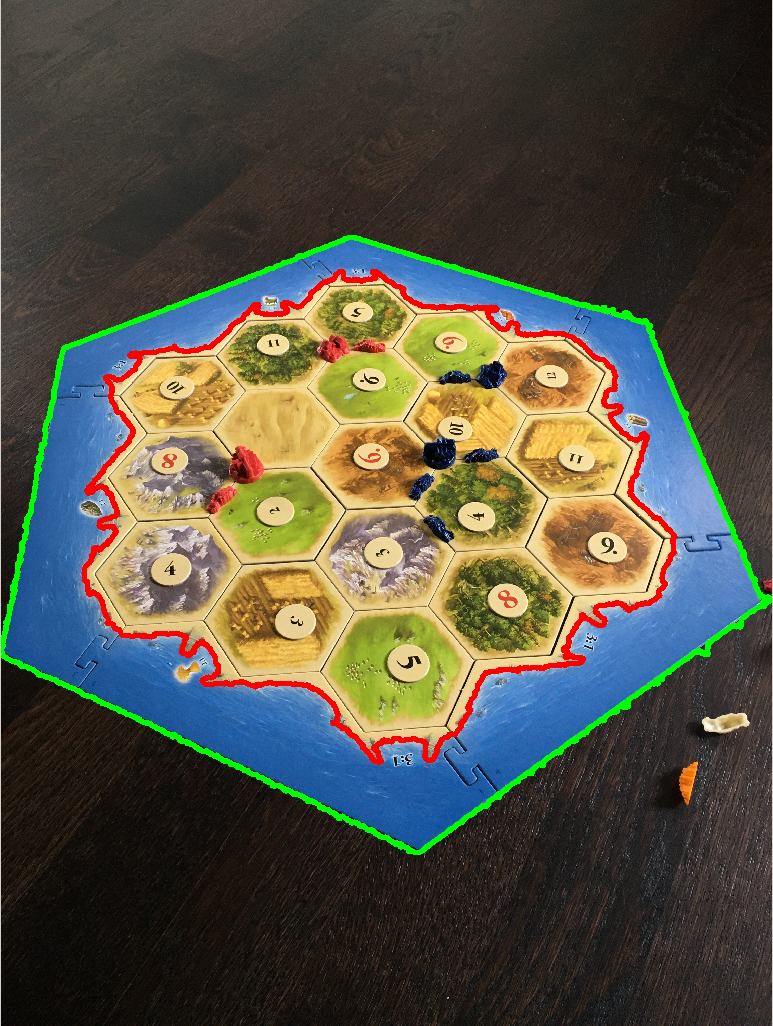
\includegraphics[width=\linewidth]{pictures/steps/two_contours.png}
            \subcaption{Dwa największe kontury}
        \end{subfigure}
        \begin{subfigure}[t]{0.32\linewidth}
            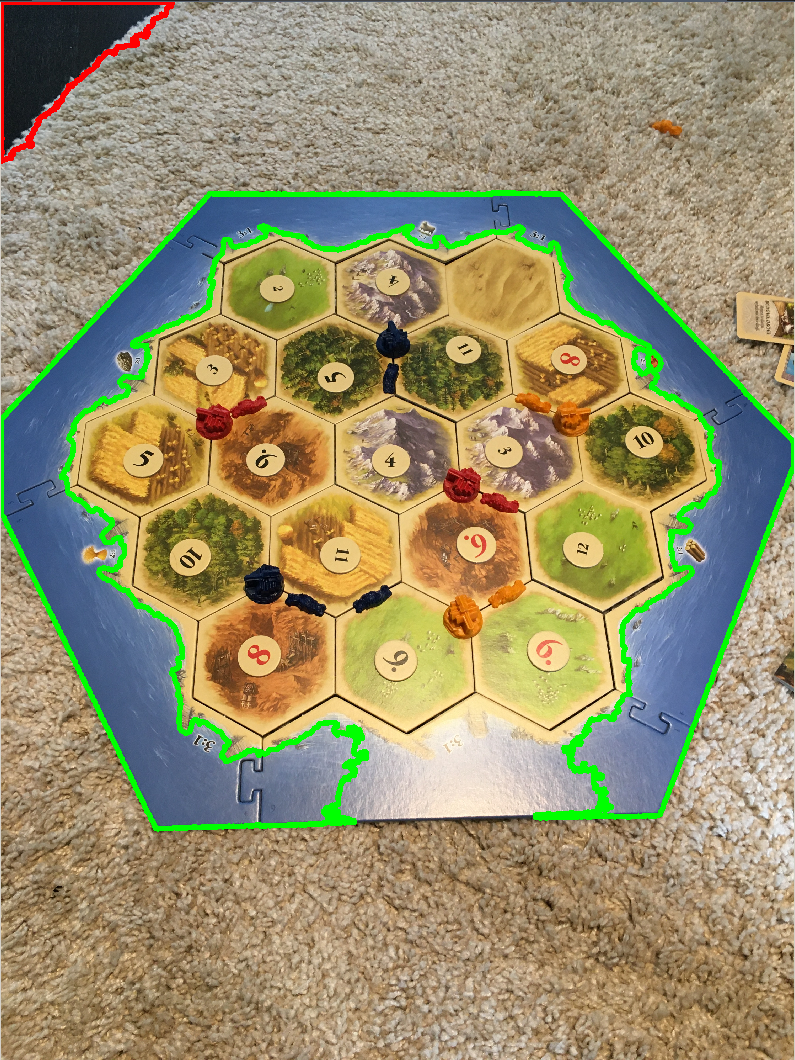
\includegraphics[width=\linewidth]{pictures/steps/two_contours_blend.png}
            \subcaption{Kontury łączą się ze sobą}
        \end{subfigure}
        \begin{subfigure}[t]{0.32\linewidth}
            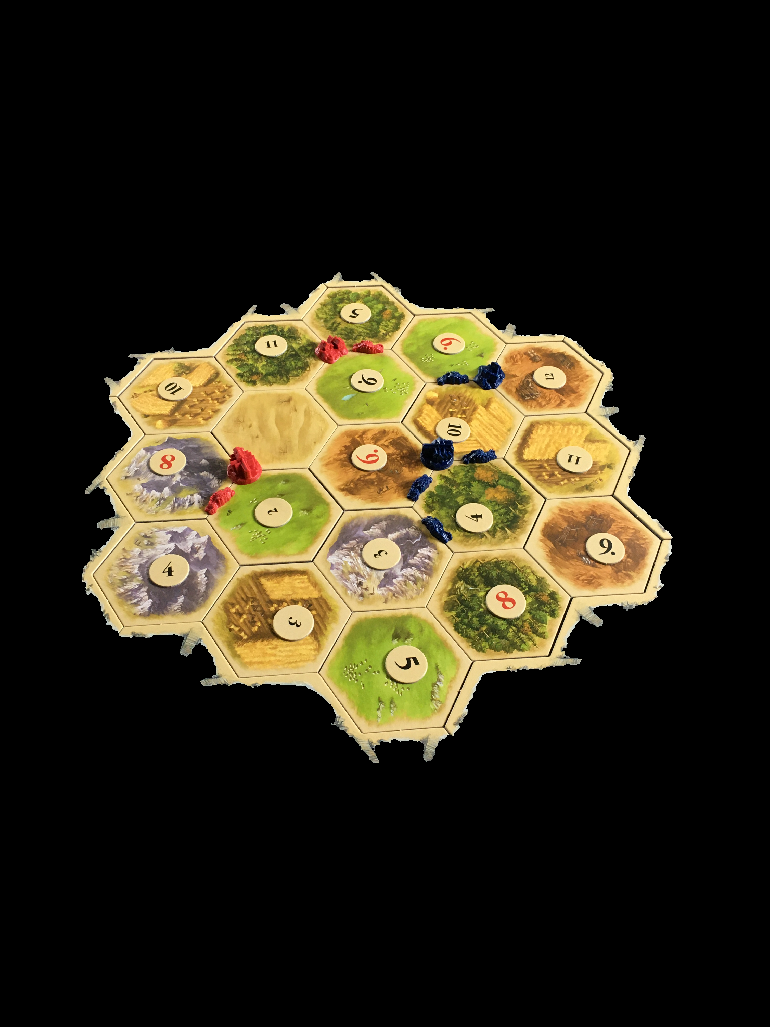
\includegraphics[width=\linewidth]{pictures/steps/background_cut.png}
            \subcaption{Wycięte tło}
        \end{subfigure}
        \caption{Wycinanie tła}
        \label{fig:step1}
    \end{figure}

    \subsection{Znajdowanie pionków}

    \subsection{Rozpoznawanie pionków}
    Na każdej masce uzyskanej w poprzednim kroku szukamy konturów. Dla każdego z nich wyznaczamy otoczkę wypukłą (convex hull), ponieważ pionki wykonane są z błyszczącego plastiku i trudno jest zapewnić, aby w całości były zaznaczone na masce.

    Następnie w każdą otoczkę, której powierzchnia znajduje się w akceptowalnym przedziale wpasowywana jest elipsa.
    Liczymy stosunek półosi wielkiej do półosi małej elipsy. Dla miast i osad stosunek ten jest bliski 1, natomiast drogi są bardziej podłużne, więc dla nich ten stosunek jest niższy.

    Jeżeli jednak powierzchnia otoczki danego konturu przekracza akceptowalną wartość, może to oznaczać, że na tym obszarze znajdują się w rzeczywistości dwa pionki. Dlatego ten kontur rysujemy na nowej, czystej masce. Maskę następnie poddajemy erozji i rekurencyjnie wywołujemy na niej funkcję rozpoznającą pionki. Robimy tak do czasu, aż powierzchnia otoczki znajdzie się w akceptowalnym przedziale.

    Dla każdego zidentyfikowanego pionka wyznaczany jest centroid, który następnie zaznaczany jest na obrazie.
    
    \subsection{Znajdowanie i rozpoznawanie pól}
      
\section{Przedstawienie wyników}
    \subsection{Zdjęcia łatwe}
    \begin{figure}[H]
        \begin{subfigure}[]{\linewidth}
            \includegraphics[width=\linewidth]{pictures/easy1.png}
            \subcaption{Brak pionków}
        \end{subfigure}

        \begin{subfigure}[]{\linewidth}
            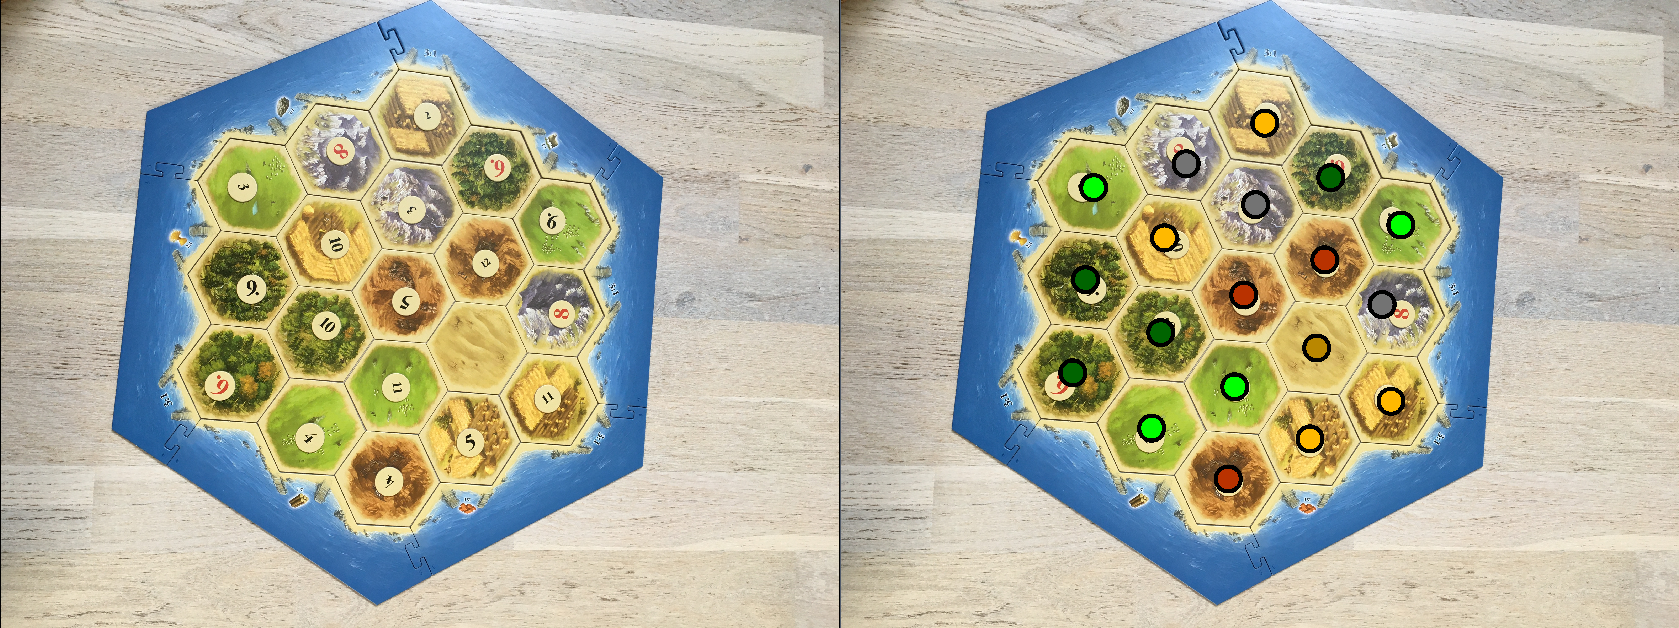
\includegraphics[width=\linewidth]{pictures/easy2.png}
            \subcaption{Liczby na planszy}
        \end{subfigure}
        \caption{Przykłady zdjęć łatwych}
        \label{fig:step1}
    \end{figure}
    
    \subsection{Zdjęcia średnie}
    \subsection{Zdjęcia trudne}
    \begin{figure}[H]
        \begin{subfigure}[]{\linewidth}
            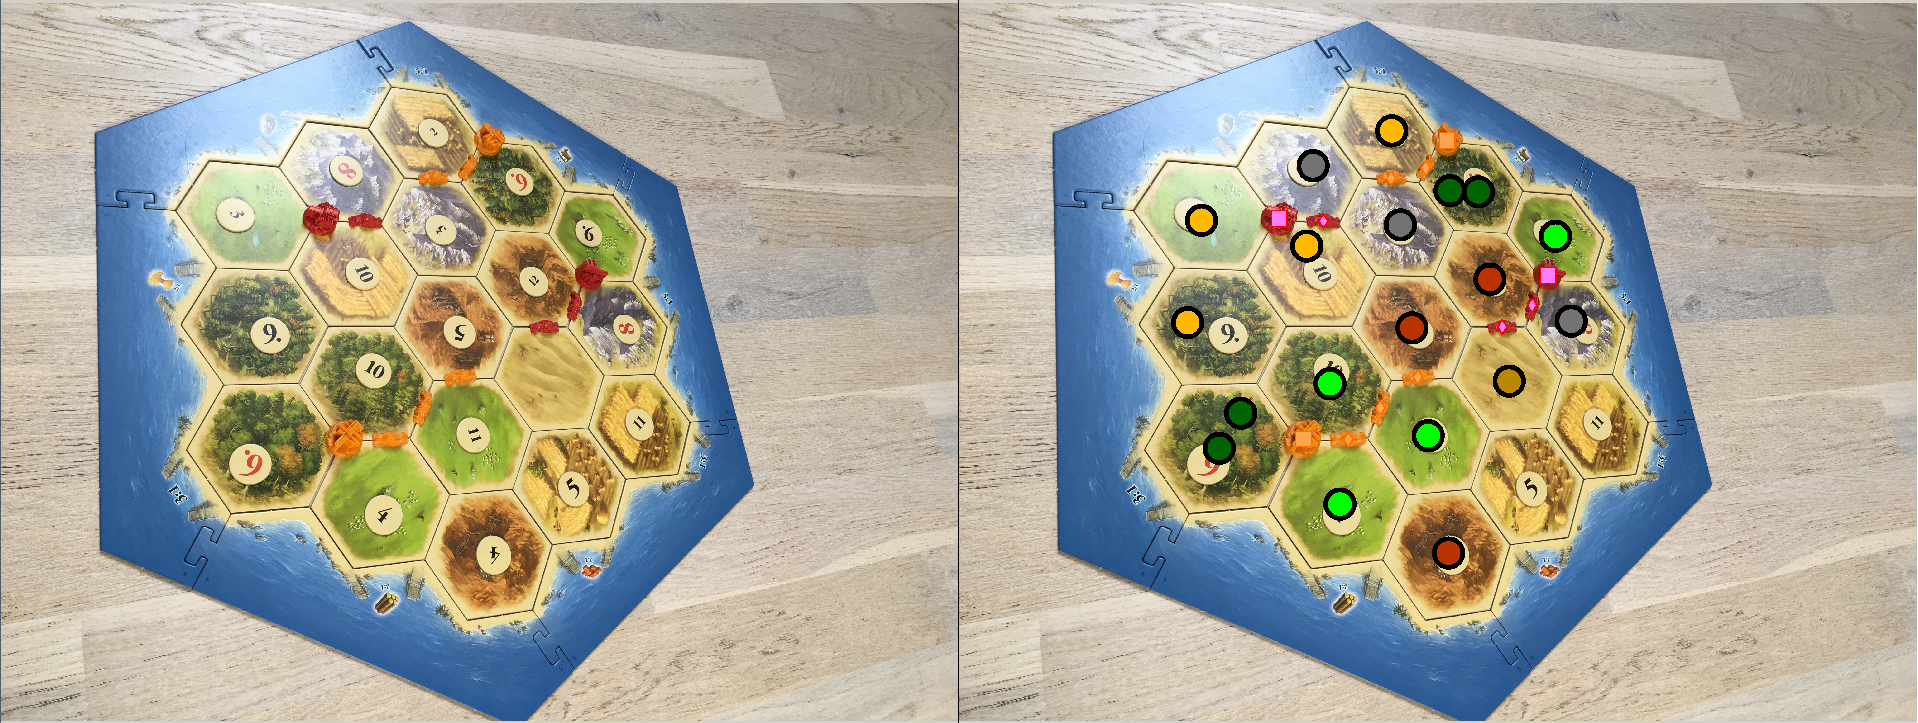
\includegraphics[width=\linewidth]{pictures/hard1.png}
            \subcaption{Prześwietlone zdjęcie}
        \end{subfigure}

        \caption{Przykłady zdjęć łatwych}
        \label{fig:step1}
    \end{figure}
\section{Podsumowanie wyników}
.

\end{document}
